\documentclass{article}
\usepackage{float}
\usepackage{amsmath}
\usepackage{longtable}
\usepackage[margin=1in]{geometry}
\usepackage{caption}
\usepackage{booktabs}
\usepackage[dvipsnames]{xcolor}
\usepackage{fancyvrb}
\usepackage{graphicx}
\RecustomVerbatimCommand{\VerbatimInput}{VerbatimInput}%
{fontsize=\footnotesize,
 %
 frame=lines,  % top and bottom rule only
 framesep=2em, % separation between frame and text
 rulecolor=\color{Gray},
 %
 label=\fbox{\color{Black}Profiling Result},
 labelposition=topline,
 %
 commandchars=\|\(\), % escape character and argument delimiters for
                      % commands within the verbatim
 commentchar=*        % comment character
}

\begin{document}
\title{STA663 Final Project \\ Indian Buffet Process and its application in the Infinite Latent Feature Model}
\author{Dipesh Gautam}
\date{\today}
\maketitle

\section{Background}
\subsection{Indian Buffet Process (IBP)}
The Indian Buffet is an adaptation of Chinese Buffett Process where each object instead of being associated with a single latent class can  be associated with multiple classes. This is particularly useful when each object has multile latent features and by associating objects with a single class we cannot partition them into homogeneous subsets.

In the Indian buffet process, $N$ customers enter a restaurant one after another. Each customer encounters a buffet 
consisting of infinitely many dishes arranged in a line. The first customer starts at the left of the buffet and 
takes a serving from each dish, stopping after a Poisson($\alpha$) number of dishes. The $i$th customer moves along the buffet, 
sampling dishes in proportion to their popularity, taking dish $k$ with probability $\frac{m_k}{i}$ , where $m_k$ is the number of 
previous customers who have sampled that dish. Having reached the end of all previous sampled dishes, the $i$th customer 
then tries a Poisson($\frac{\alpha}{i}$) number of new dishes. Which costumer chose which dishes is indicated using a binary matrix \textbf{Z} with $N$ rows and infinitely many columns(corresponding to the infinitely many selection of dished), where $z_{ik}$ = 1 if the $i$th costumer sampled $k$th dish.

IBP can be used as a prior in models for unsupervised learning. An example of which is presentd in the paper by Griffiths and Ghahramani, where IBP is used as a prior in linear-Gaussian binary latent feature model.


\section{Implementation}
\subsection{Infinite Latent Features Model and Algorithm}
\begin{itemize}
\item{Gamma prior for $\alpha$
$$
\alpha \sim Gamma(1,1)
$$}
\item{Prior on \textbf{Z} is obtained by IBP as:
$$
P(z_{ik}=1|\textbf{z}_{-i,k}) = \frac{n_{-i,k}}{N}
$$}

\item{Likelihood is given by
\begin{equation}
P(X|Z,\sigma_X, \sigma_A) = \frac{1}{(2 \pi)^{ND/2} (\sigma_X)^{(N-K)D}(\sigma_A)^{KD}(|Z^TZ+\frac{\sigma_X^2}{\sigma_A^2}I|)^{D/2}}exp\{-\frac{1}{2\sigma_X^2}tr(X^T(I-Z(Z^TZ+\frac{\sigma_X^2}{\sigma_A^2}I)^{-1}Z^T)X)\}
\end{equation}
}
After we have the likelihood and the prior given by IBP,
\item{full conditional posterior for \textbf{Z} can be calculated as:
$$
P(z_{ik}|X,Z_{-(i,k)},\sigma_X,\sigma_A) \propto  P(X|Z,\sigma_X, \sigma_A) * P(z_{ik}=1|\textbf{z}_{-i,k}) 
$$
}

To sample the number of new features for observation $i$, we use a truncated distribution, computing probabilities for a range of values $K_1^{(i)}$ up to an upper bound (say 4). The prior on number of features is given by $Poisson(\frac{\alpha}{N})$.
Using this prior and the likelihood, we sample the nummber of new features.

\item{Full conditional posterior for $\alpha$ is given by:
$$
P(\alpha|Z) \sim Gamma(1+K_+,1+\sum_{i=1}^{N} H_i)
$$}

\item{For $\sigma_X$ and $\sigma_A$, we use MH algorithm as follows:
\begin{eqnarray}
\epsilon \sim Uniform(-.05,.05)\\
\sigma_X^{*} =  \sigma_X +\epsilon\\
\end{eqnarray}
Accept this new $\sigma_X$ with probability given by:
$$
AR = min\{1,\frac{Likelihood(X|\sigma_X^{\*},...)}{Likelihood(X|\sigma_X,...)}\}\\
$$
Where AR is the acceptance ratio. We use similar algorithm to sample $\sigma_A$}

\end{itemize}

\subsection{Simulated Data}


\subsection{Unit Testing}


\section{Profiling and Optimization}
We profiled the code using \textit{cProfile} to figure out bottlenecks. The result is shown in \textit{Profiling result}. We see that most of the computational time is spent on calculating the \textit{log likelihood(ll)}  and matrix inversion. Due to this fact, one of the first things we looked at were ways to reduce computation time for likelihood and/or inverse calculation.\\

\VerbatimInput{profiler.txt}

\subsection{Matrix Inversion}
We tried the matrix inversion method described in Griffiths and Ghahramani(2005, eq 51-54), where the method reduces the runtime by allowing us to perform rank one updates instead when only one value is changed. We implemented the algorithm and were able to speed up the process as shown in Table \ref{compareInverse}.

\begin{table}[ht]
\centering
\caption{Comparision of matrix inverse methods \label{compareInverse}}
\begin{tabular}{lr}
\toprule
{} &      Time \\
\midrule
linalg.inverse &  0.000078 \\
calcInverse    &  0.000036 \\
\bottomrule
\end{tabular}

\end{table}

Even though we were able to improve the performance, due to some numerical errors, we were not able to obtain a stationary MCMC chain using this method. This could be achieved by spending some more time on it but due to time constraints we decided that to look at fixing this at a later time.\\

\subsection{Likelihood function}
While working on the optimized matrix inversion, we noticed that the matrix that we're inverting i.e. ($Z^TZ+\frac{\sigma_X^2}{\sigma_A^2}I$) actually appears twice inside the likelihood function. So, we looked at removing the redundancy by calculating the matrix and storing it. We were able to gain some improvement using this method as shown in Table \ref{llcomp} and Table \ref{runtimes}. Since the likelihood function is called numerous times, even the small gain shwon in Table \ref{llcomp} was translated into a substantial gain as shown in Table \ref{runtimes}.\\


\begin{table}[H]
\centering
\caption{Runtime Comparision \label{llcomp}}
\begin{tabular}{lr}
\toprule
{} &      Time \\
\midrule
original ll function &  0.000392 \\
Proposed ll function &  0.000337 \\
\bottomrule
\end{tabular}


\end{table}

\subsection{Cython}
Another way we looked at improving the performance of the code was by cythonizing the code. We again looked at improving the performance of the likelihood function by cythonizing it. As shwon in Table \ref{runtimes}, we were not able to gain substantial improvements from it.\\


\subsection{Parallelization and CUDA}
Since our algorithm is an MCMC algorithm with serial dependence, parallelization does not seem to be a good idea. One of the ways, parallelization can be done is by splitting the chain into multiple smaller chains and combining them back. We tested it and it showed some improvement in the code but decided against using it as the gain wasn't significant enough as we had to take care of multiple burn-in periods and ignore the loss of markov property due to multiple chains. Also, parallelizing the density calculation for likelihood wasn't an option for our algorithm as we had a discrete density with just two points.


\begin{table}[ht]
\centering
\caption{Runtime Comparision \label{runtimes}}
\begin{tabular}{lr}
\toprule
{} &  Total Time \\
\midrule
Initial Code &  539.818143 \\
Improved ll  &  489.207815 \\
Cythonized   &  507.522965 \\
\bottomrule
\end{tabular}

\end{table}



\begin{figure}
\caption {Original Features and First four simulated objects}
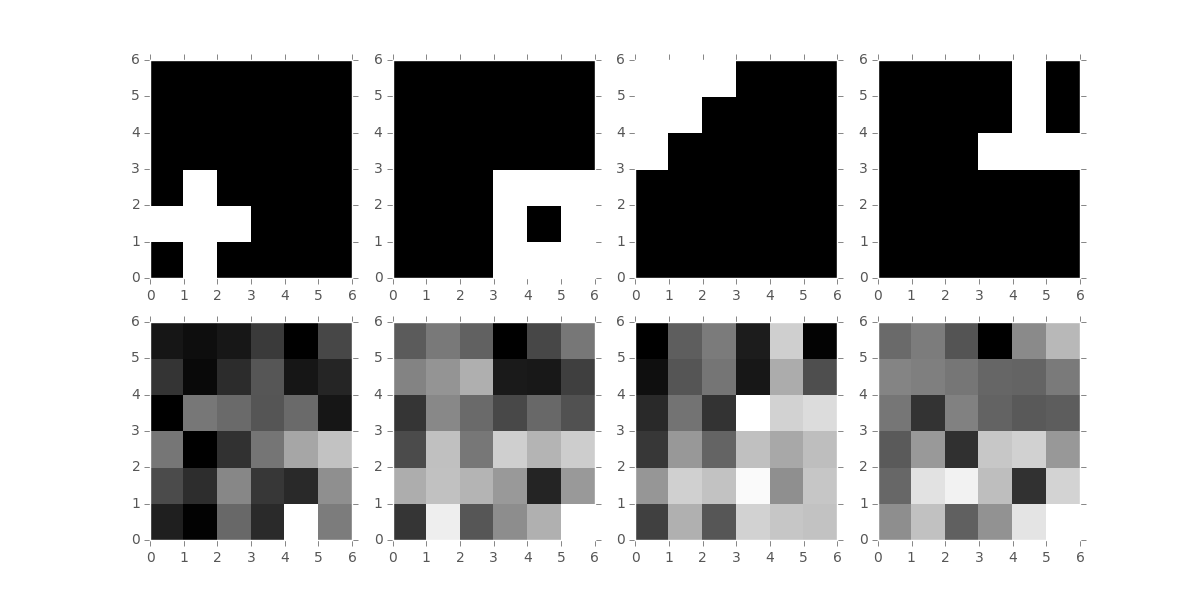
\includegraphics[width=\linewidth]{figures/Original.png}
\label{fig:original}
\end{figure}



\begin{figure}
\caption {Features Detected after MCMC and First four recreated objects}
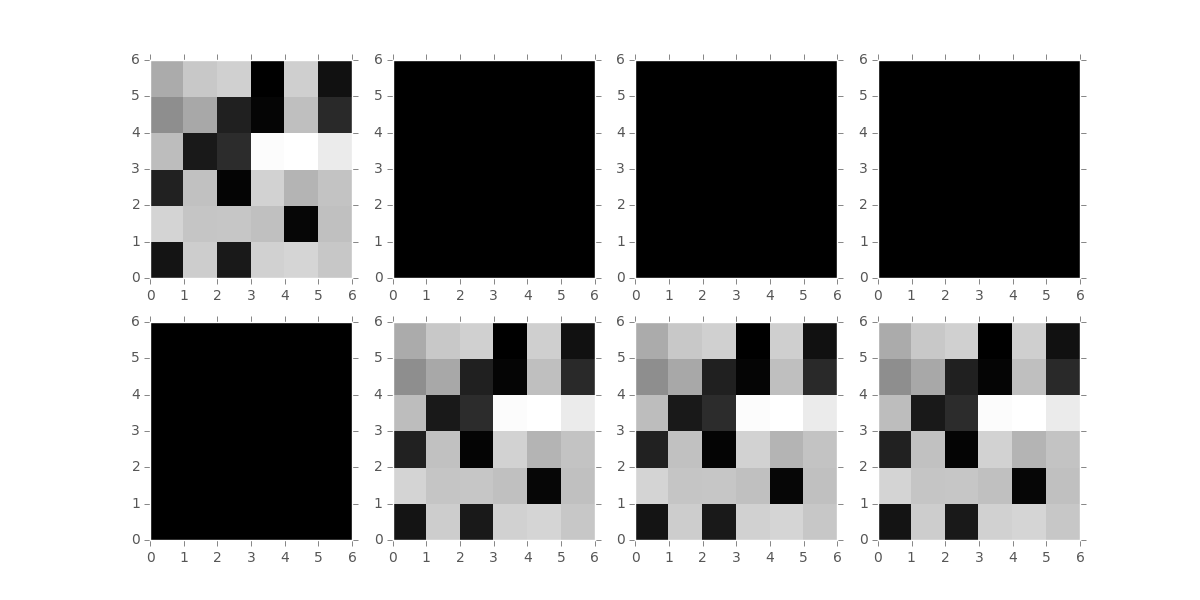
\includegraphics[width=\linewidth]{figures/Detected.png}
\label{fig:detected}
\end{figure}

\begin{figure}
\caption {Traceplots for $\sigma_X$, $\sigma_A$ and $\alpha$ after burn-in}
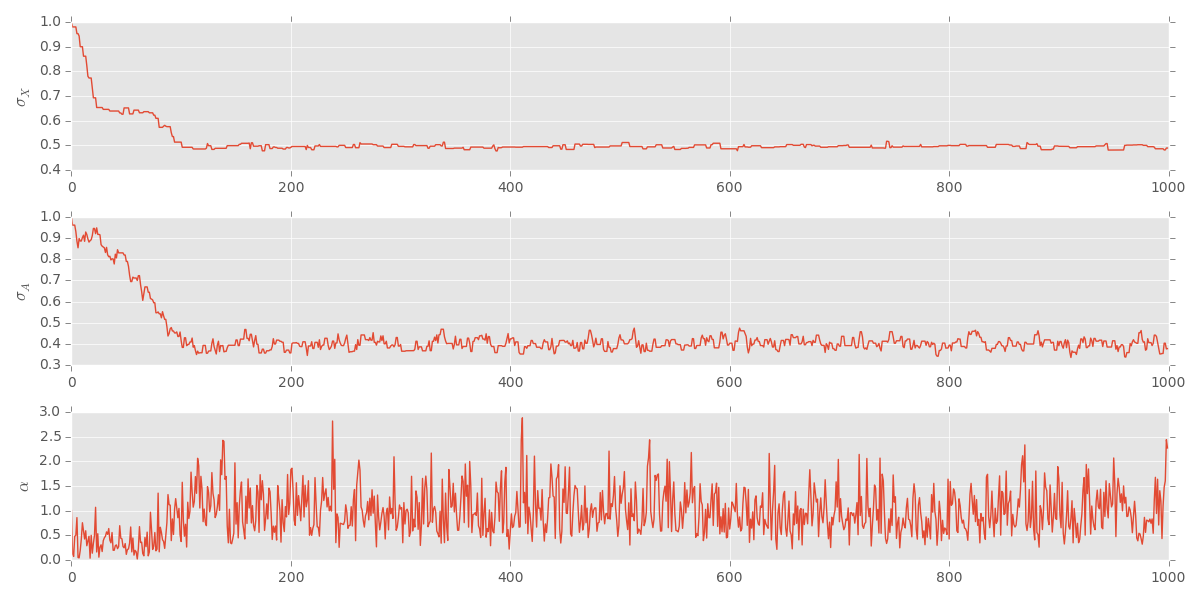
\includegraphics[width=\linewidth]{figures/Trace.png}
\label{fig:trace}
\end{figure}

\begin{figure}
\caption {Distribution of Kplus}
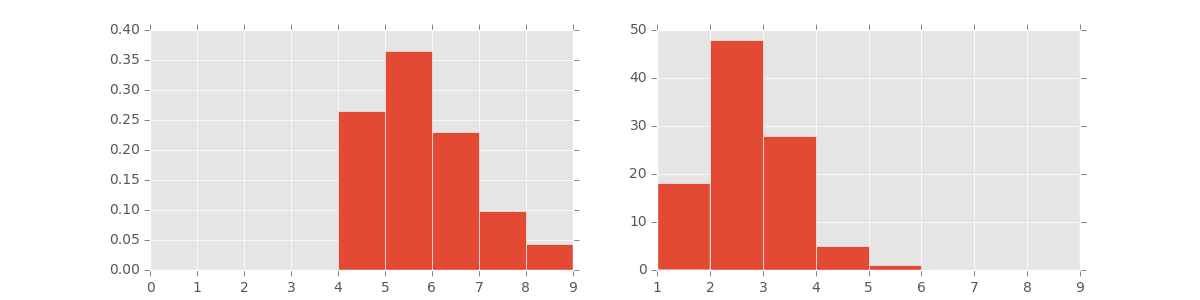
\includegraphics[width=\linewidth]{figures/kDistribution.png}
\label{fig:dist}
\end{figure}

\begin{table}[ht]
\centering
\caption{Features present in first four original images \label{features}}
\begin{tabular}{lrrrr}
\toprule
{} &  F1 &  F2 &  F3 &  F4 \\
\midrule
1st image &   0 &   1 &   0 &   0 \\
2nd image &   1 &   1 &   0 &   0 \\
3rd image &   1 &   1 &   0 &   1 \\
4th image &   1 &   1 &   0 &   0 \\
\bottomrule
\end{tabular}

\end{table}





\end{document}
